\chapter{Self-Supervised Attribution} \label{ch:method}



\section{Formalization} \label{sec:problem}

The idea behind the method proposed in this thesis relies on the assumption that the relevant features that result in the prediction of a given output also allow the same outcome to be predicted if isolated from the original full input. Building on top of this assumption, the intuition is that an explanation can be learned in a self-supervised manner by enforcing the predicted attribution maps to preserve the original performance of the model.

Formally, given a model to explain $f$, the problem we aim to solve is the following:
\begin{equation} \label{eq:problem1}
    \min_{\S \in [0, 1]^{N}} \left\Vert f(\x) - f(\x \otimes \S) \right\Vert + \gamma \left\Vert \S \right\Vert,
\end{equation}
where:
\begin{itemize}
    \item $\S$ is the attribution map we aim to find,
    \item $N$ is the size of the input space,
    \item $\x$ is the input of the model $f$,
    \item $\otimes$ denotes the operation of applying the attribution map $\S$ on the input $\x$. In our case, we use the product and $\S$ can be interpreted as a weight of the input.
\end{itemize}
In this formulation of the problem, the first term imposes that the outcome of the model where the input is filtered based on the attribution scores should be close to the one using the full input, while the second term encourages sparsity in attribution scores and avoids the trivial solution where $\S$ is a matrix of ones.

As is, the current formulation of the problem defines a model-agnostic method for explainability. In this thesis, we consider the case where $f$ is a neural network. This allows us to approach the problem from a different perspective by replacing the first term in \Cref{eq:problem1} with the loss function $\L$ used to train $f$. Therefore, the resulting problem becomes:
\begin{equation}
    \min_{\S \in [0, 1]^{N}} \L(\x \otimes \S; f) + \gamma \left\Vert \S \right\Vert.
\end{equation}
In other words, in the case of neural networks, the problem of maintaining the same output of the original input can be reduced to the problem of preserving the loss function when using the filtered input.



\section{Architecture}

In practical terms, we solve the problem described in \Cref{sec:problem} by introducing a new model on top of the existing one. In this work, we focus on explaining traditional fine-tuned classifiers composed of a feature encoder and a classification head. The overall idea of the architecture is depicted in \Cref{fig:training}.

\begin{figure}[t!]
    \centering
    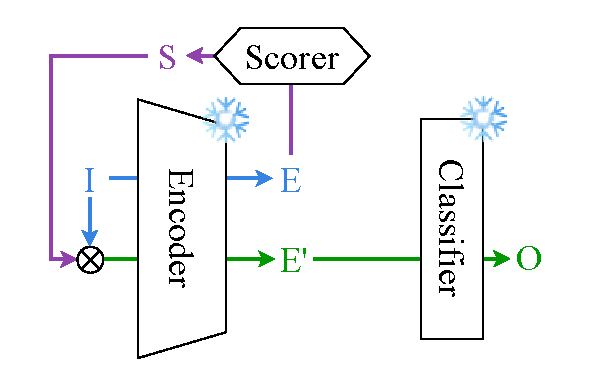
\includegraphics[scale=0.65]{./img/idea.pdf}
    \caption{General idea of the method. Given a traditional classifier (encoder and classification head), we introduce a new module (scorer) that learns to score the input $I$ of the encoder given its embeddings $E$.} \label{fig:training}
\end{figure}

\begin{figure}[t!]
    \centering
    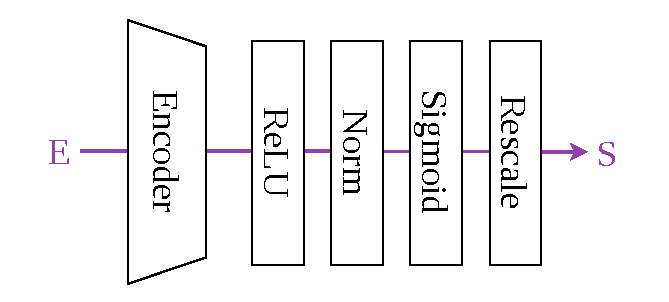
\includegraphics[scale=0.65]{./img/scorer-arch.pdf}
    \caption{Architecture of the scorer} \label{fig:scorer}
\end{figure}

The flow between the encoder and the classifier is as usual. The newly introduced model, called scorer for simplicity, should take as input some information of the input features of the explainee model and it outputs a score for each of them. In case of classifiers, we use the embedding space of the encoder as inputs for the scorer.

We also note that in principle we could provide to the scorer the original input itself. Intuitively, this formulation would still allow to learn some reasonable attribution maps that highlight what is relevant in the input as the goal is still to minimize the task specific loss. However, it would require the scorer to solve the whole classification task as well and no signal from the target model to explain would be included in the flow, so the result of this setup would be closer to an explainable-by-design model.

In terms of architecture, a crucial choice for the scorer, although unusual, is how its output head is designed. A high-level depiction of the architecture is provided in \Cref{fig:scorer}. The scorer itself contains an encoder to refine the input and the output activations it produces are passed through: 
\begin{enumerate*}
    \item a rectified linear unit (ReLU) activation, 
    \item a sigmoid activation, and 
    \item rescaled into $[0, 1]$ . 
\end{enumerate*}
The ReLU activation is used to impose a strong distinction between relevant signal (activation greater than $0$) and background that is not useful for the attribution map. The sigmoid function squeezes the scores into $[0, 1]$ and adds a further level of non-linearity, and the final rescaling actually ensures that the scores span from $0$ to $1$.



\section{Training and Inference}

The scorer module introduced to compute attribution scores is implemented as a neural network and therefore requires training. As we aim at solving the problem defined in \Cref{sec:problem}, we can reformulate it to an optimization problem that can be used to train neural networks. Therefore, we can define the loss function as the following:
\begin{equation}
    \label{eq:loss_naive}
    \begin{aligned}
        \L(\x, \S; f) =\,\, &\L_\text{task}(\x \otimes \S; f) \\
        &+ \gamma_1 \left( \frac{1}{\vert \S \vert} \sum_i^{\vert S \vert} s_i \right)^2 \\
        &+ \gamma_2 \frac{1}{\vert \S \vert} \sum_i^{\vert S \vert} (s_i \cdot (1-s_i))^2 \\
    \end{aligned}
\end{equation} 
where $\L_\text{task}$ is the task-specific loss (cross-entropy in our case), the first penalty term encourages sparsity in the attribution scores so that few positions have high values, and the second penalty term is for pushing scores to be closer to either $0$ or $1$ so that it is more similar to a binary mask. $\gamma_1$ and $\gamma_2$ are instead hyperparameters to weight the importance of the two penalties. 

Ideally, we would like to avoid having to choose and tune arbitrary hyperparameters such as $\gamma_1$ and $\gamma_2$. It turns out that, by how the problem is posed, it is possible to define these two hyperparameters in such a way that they are self-calibrating. We are able to do this by exploiting the information we have about the loss function during training. The idea is to use the inverse distance between the loss evaluated with the masked input and the original one as the weight for the penalties. In this way, the intuition is that when the produced attribution map is preserving the loss, the weight of the penalties can be increased, while if the original loss is not preserved, the penalties are down-weighted so that the learning process can focus on preserving the original capabilities first without being drifted away by the penalties. Therefore, our final training loss is defined as follows:
\begin{equation}
    \label{eq:loss}
    \begin{gathered}
        \begin{aligned}
            \L(\x, \S; f) =\,\, &\L_\text{task}(\x \otimes \S; f) \\
            &+ \gamma \left( \frac{1}{\vert \S \vert} \sum_i^{\vert S \vert} s_i \right)^2 \\
            &+ \gamma \frac{1}{\vert \S \vert} \sum_i^{\vert S \vert} (s_i \cdot (1-s_i))^2 \\
        \end{aligned} \\
        \text{with } \gamma = \texttt{clip}\left\{ \frac{1}{\L_\text{task}(\x \otimes \S; f) - \L_\text{task}(\x; f) + \varepsilon}, [0, 1] \right\},
    \end{gathered}
\end{equation}
where $\gamma$ is the self-calibrating weight based on the distance between losses and $\texttt{clip}$ constrains the weight in $[0, 1]$ to avoid having values that grow uncontrollably, which would make the penalties reach unreasonably high magnitudes, or that go below zero, which would have the opposite effect we aim at achieving.

In terms of parameter updates, we must note that this method does not require to modify the target model as its weights are kept frozen when training the scorer, as depicted in \Cref{fig:training}. This avoids leaking any relevant information for the scorer into the original classifier, so that we can ensure that what it learns is to actually provide attribution maps for the target model without any shortcut. 

\begin{figure}[t!]
    \centering
    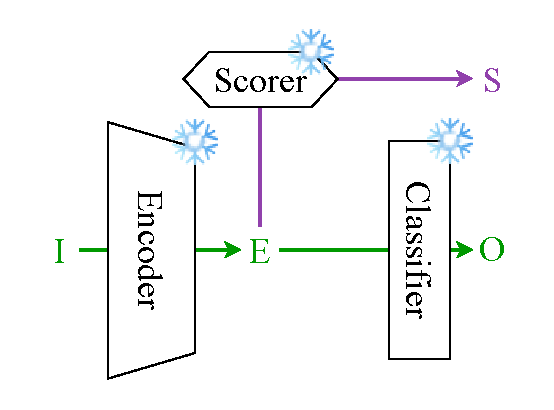
\includegraphics[scale=0.65]{./img/inference.pdf}
    \caption{At inference time, the flow of the classifier is unaffected by the scorer. The output of the scorer corresponds to the attribution map.} \label{fig:inference}
\end{figure}

At inference time, as depicted in \Cref{fig:inference}, this method works transparently alongside the existing classification model. It does not disrupt any of its normal flow and only uses some intermediate information provided by the encoder that is fed into the scorer to determine the output attribution scores.


\subsection{Text Modality} \label{sec:text_scorer}

For text classification, we consider the standard approach based on tokenizing the text sequence and mapping it to embeddings \cite{text_survey_2022}. The flow of the classification model is therefore the following:
\begin{enumerate*}
    \item split sentence into tokens according to a vocabulary,
    \item embed each token based on some static embeddings,
    \item refine the initial embeddings through the text encoder,
    \item pool the resulting embeddings and pass through the classifier.
\end{enumerate*}
The embeddings at step (c) are the most information rich and can be used as the input of the scorer that produces a score for each input token. At training time, as depicted in \Cref{fig:training_text}, we apply these scores to weigh the static embeddings at step (b) before passing them through the encoder. This choice is motivated by two aspects: on the one hand, as we need to integrate the learned attribution maps into the training process, we have to apply the scores at some stage where the input is differentiable and, as the input tokens are discrete and non-differentiable, the first layer at which this is possible is after applying the static embeddings. On the other hand, applying the learned attribution maps on the embeddings produced by the final text encoder would have the risk of being ineffective as each token already had the opportunity to interact with each other first which would make masking an embedding not the same as masking an input token. 

\begin{figure}[t!]
    \begin{subfigure}[b]{0.49\textwidth}
        \centering
        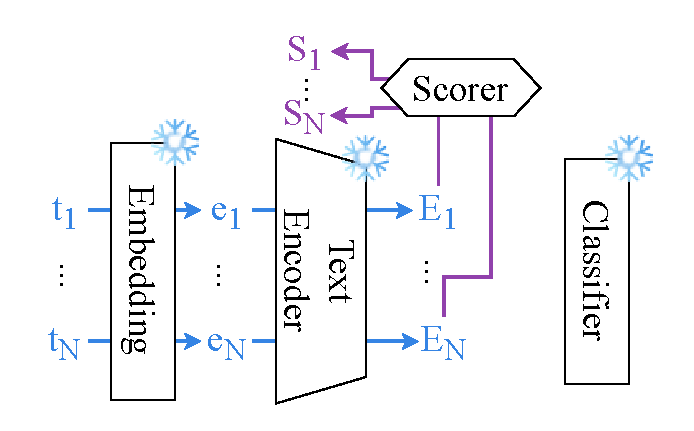
\includegraphics[scale=0.6]{./img/arch-text1.pdf}
        \caption{}
    \end{subfigure}
    \quad
    \begin{subfigure}[b]{0.49\textwidth}
        \centering
        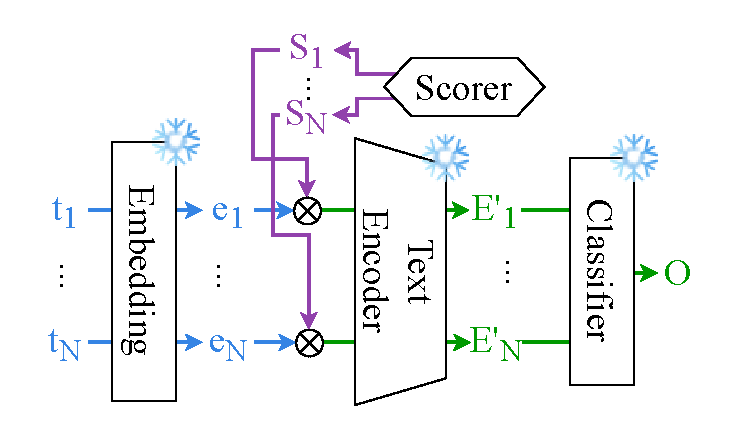
\includegraphics[scale=0.6]{./img/arch-text2.pdf}
        \caption{}
    \end{subfigure}
    \caption{Training architecture for text classifiers} \label{fig:training_text}
\end{figure}



\subsection{Image Modality} \label{sec:image_scorer}

\begin{figure}[t!]
    \centering
    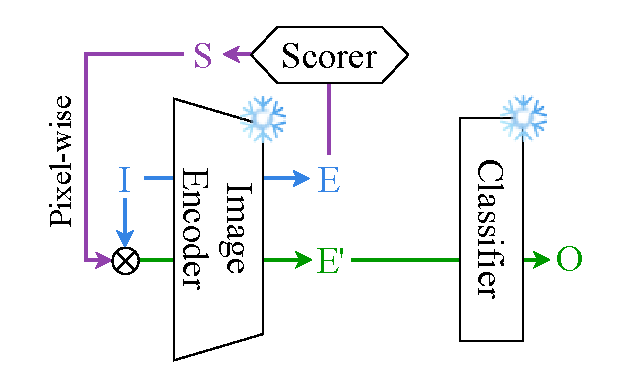
\includegraphics[scale=0.65]{./img/arch-image.pdf}
    \caption{Training architecture for image classifiers} \label{fig:training_image}
\end{figure}

For image classification, we use the traditional approach consisting of an image encoder with a classification head \cite{image_survey_2022}. The flow of the classification model is therefore the following:
\begin{enumerate*}
    \item embed the input image with the encoder,
    \item pool the resulting embeddings and pass through the classifier.
\end{enumerate*}
The embeddings at step (a) can be used as the input of the scorer that produces a score for each input pixel. At training time, as depicted in \Cref{fig:training_image}, we apply these scores to weigh each pixel of the input image before passing them through the encoder. Differently from text, in this case we do not need to add any additional considerations as the input image is already differentiable and the whole process can be directly integrated into the training process.


\subsection{Multimodality}

\begin{figure}[t!]
    \centering
    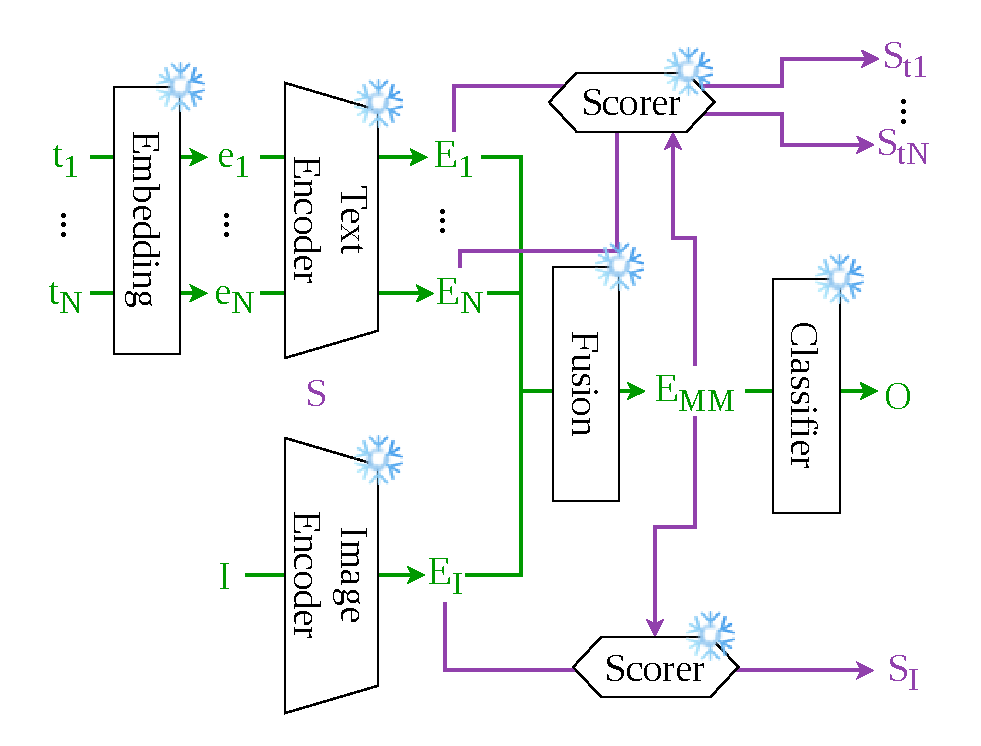
\includegraphics[scale=0.6]{./img/arch-multi.pdf}
    \caption{Inference for text-image classifiers} \label{fig:inference_multi}
\end{figure}

When moving to multimodal models, we can naturally extend our idea by combining the two scorers for text and image as we described in \Cref{sec:text_scorer,sec:image_scorer}. We depict this idea in \Cref{fig:inference_multi} for the case of text-image models. Additionally, in the case of multimodal models, the output of the two encoders are merged through a fusion layer \cite{fusion}, which stays frozen as the rest of the classifier. To avoid losing cross-modality information, the scorers in the multimodal case also take, alongside the embeddings of their modality, the output produced by the fusion layer as conditioning. The loss function is also modified to account for the two scorers: firstly, by extending \Cref{eq:loss} to the multimodal case, we evaluate the cross-entropy loss with both text and image masked so that the scorers are encouraged to preserve the original model. Secondly, to make the task easier and guide the learning process, we also minimize the cross-entropy of the two modalities separately by masking only either the text or the image. Thirdly, as there are two scorers, we introduce two sets of penalties to also handle the attribution maps produced by the two modalities separately. Therefore, after training the target multimodal classifier, we keep both encoders, the fusion layer, and the classification head frozen. Then, we train the two scorers by optimizing the following function:
\begin{equation}
    \begin{gathered}
        \begin{aligned}
            \L(\x_1|\x_2, \S_1|\S_2; f) =\,\, 
            & \L_\text{task}(\x_1 \otimes \S_1 | \x_2 \otimes \S_2; f) \\
            &+ \L_\text{task}(\x_1 \otimes \S_1 | \x_2; f) + \L_\text{task}(\x_1 | \x_2 \otimes \S_2 ; f)\\
            &+ \gamma \left( \frac{1}{\vert \S_1 \vert} \sum_i^{\vert S_1 \vert} s_{1,i} \right)^2 
             + \gamma \left( \frac{1}{\vert \S_2 \vert} \sum_j^{\vert S_2 \vert} s_{2,j} \right)^2 \\
            &+ \gamma \frac{1}{\vert \S_1 \vert} \sum_i^{\vert S_1 \vert} (s_{1,i} \cdot (1-s_{1,i}))^2
             + \gamma \frac{1}{\vert \S_2 \vert} \sum_j^{\vert S_2 \vert} (s_{2,j} \cdot (1-s_{2,j}))^2 \\
        \end{aligned} \\
        \text{with } \gamma = \frac{1}{\texttt{clip}\{ \L_\text{task}(\x_1 \otimes \S_1 | \x_2 \otimes \S_2; f) - \L_\text{task}(\x_1|\x_2; f), [0, 1] \}},
    \end{gathered}
\end{equation}
where:
\begin{itemize}
    \item $\x_1$ and $\x_2$ are the inputs of the two modalities,
    \item $\S_1$ and $\S_2$ are the attribution scores of the two modalities,
    \item $\gamma$ is the self-calibrating parameter based on the logits obtained by masking both modalities.
\end{itemize}
